\documentclass{beamer}

\usepackage{beamerthemesplit}
\usepackage{graphicx}
\usepackage{color, natbib, hyperref}
\usepackage{bibentry}
\nobibliography*

% define colors
\definecolor{jblue}  {RGB}{20,50,100}
\definecolor{ngreen} {RGB}{98,158,31}

%theme

\usetheme{boxes} 
%\usecolortheme{seahorse} 
\setbeamertemplate{items}[default] 
%\setbeamercovered{transparent}
\setbeamertemplate{blocks}[rounded]
\setbeamertemplate{navigation symbols}{} 
% set the basic colors
\setbeamercolor{palette primary}   {fg=black,bg=white}
\setbeamercolor{palette secondary} {fg=black,bg=white}
\setbeamercolor{palette tertiary}  {bg=jblue,fg=white}
\setbeamercolor{palette quaternary}{fg=black,bg=white}
\setbeamercolor{structure}{fg=jblue}
\setbeamercolor{titlelike}         {bg=jblue,fg=white}
\setbeamercolor{frametitle}        {bg=jblue!10,fg=jblue}
\setbeamercolor{cboxb}{fg=black,bg=jblue}
\setbeamercolor{cboxr}{fg=black,bg=red}

% reduce space before/after equations
\expandafter\def\expandafter\normalsize\expandafter{%
    \normalsize
    \setlength\abovedisplayskip{1pt}
    \setlength\belowdisplayskip{1pt}
    \setlength\abovedisplayshortskip{1pt}
    \setlength\belowdisplayshortskip{1pt}
}

% set colors for itemize/enumerate
\setbeamercolor{item}{fg=ngreen}
\setbeamercolor{item projected}{fg=white,bg=ngreen}

% set colors for blocks
\setbeamercolor{block title}{fg=ngreen,bg=white}
\setbeamercolor{block body}{fg=black,bg=jblue!10}

% set colors for alerted blocks (blocks with frame)
\setbeamercolor{block alerted title}{fg=white,bg=jblue}
\setbeamercolor{block alerted body}{fg=black,bg=jblue!10}
\setbeamercolor{block alerted title}{fg=white,bg=dblue!70} % Colors of the highlighted block titles
\setbeamercolor{block alerted body}{fg=black,bg=dblue!10} % Colors of the body of highlighted blocks

% set the fonts
\usefonttheme{professionalfonts}

\setbeamerfont{section in head/foot}{series=\bfseries}
\setbeamerfont{block title}{series=\bfseries}
\setbeamerfont{block alerted title}{series=\bfseries}
\setbeamerfont{frametitle}{series=\bfseries}
\setbeamerfont{frametitle}{size=\Large}
\setbeamerfont{block body}{series=\mdseries}
\setbeamerfont{caption}{series=\mdseries}
\setbeamerfont{headline}{series=\mdseries}


% set some beamer theme options
\setbeamertemplate{title page}[default][colsep=-4bp,rounded=true]
\setbeamertemplate{sections/subsections in toc}[square]
\setbeamertemplate{items}[circle]
\setbeamertemplate{blocks}[width=0.0]
\beamertemplatenavigationsymbolsempty

% Making a DAG
\usepackage{tkz-graph}  
\usetikzlibrary{shapes.geometric}
\tikzstyle{VertexStyle} = [shape            = ellipse,
                               minimum width    = 6ex,%
                               draw]
 \tikzstyle{EdgeStyle}   = [->,>=stealth']      


% Math macros
\newcommand{\cD}{{\mathcal D}}
\newcommand{\cF}{{\mathcal F}}
\newcommand{\todo}[1]{{\color{red}{TO DO: \sc #1}}}

\newcommand{\reals}{\mathbb{R}}
\newcommand{\integers}{\mathbb{Z}}
\newcommand{\naturals}{\mathbb{N}}
\newcommand{\rationals}{\mathbb{Q}}

\newcommand{\ind}[1]{1_{#1}} % Indicator function
\newcommand{\pr}{\mathbb{P}} % Generic probability
\newcommand{\ex}{\mathbb{E}} % Generic expectation
\newcommand{\var}{\textrm{Var}}
\newcommand{\cov}{\textrm{Cov}}

\newcommand{\normal}{N} % for normal distribution (can probably skip this)
\newcommand{\eps}{\varepsilon}
\newcommand\independent{\protect\mathpalette{\protect\independenT}{\perp}}
\def\independenT#1#2{\mathrel{\rlap{$#1#2$}\mkern2mu{#1#2}}}

\newcommand{\convd}{\stackrel{d}{\longrightarrow}} % convergence in distribution/law/measure
\newcommand{\convp}{\stackrel{P}{\longrightarrow}} % convergence in probability
\newcommand{\convas}{\stackrel{\textrm{a.s.}}{\longrightarrow}} % convergence almost surely

\newcommand{\eqd}{\stackrel{d}{=}} % equal in distribution/law/measure
\newcommand{\argmax}{\arg\!\max}
\newcommand{\argmin}{\arg\!\min}


\mode<presentation>

\title[Model-based matching]{Model-based matching for causal inference in observational studies}
\author{Kellie Ottoboni \\ with Philip B. Stark and Jasjeet Sekhon}
\institute[]{Department of Statistics, UC Berkeley\\Berkeley Institute for Data Science}
\date{March 10, 2016}

\begin{document}

\frame{\titlepage}

%\AtBeginSection[]
%{
%   \begin{frame}
%       \frametitle{Outline}
%       \tableofcontents[currentsection]
%   \end{frame}
%}



\section[Introduction]{Introduction}
\frame
{
\frametitle{Observational Studies vs Experiments}

\begin{center}
\begin{itemize}
\item \textbf{Problem:} Estimate the causal effect of a treatment on outcome of interest
\item In randomized experiments, treatment is assigned to individuals at random.
\item In observational studies, the way individuals select into treatment groups is unknown.
\end{itemize}

\begin{figure}[h]
\begin{tikzpicture}
\SetGraphUnit{2} 
\Vertex{Outcome} \NOWE(Outcome){Treatment} \NOEA(Outcome){Confounder}
\Edges[color=red, label=?](Treatment, Outcome) \Edges(Confounder, Outcome) \pause \Edges(Confounder, Treatment) 
\end{tikzpicture}
\end{figure}
\end{center}
}


\frame{
\frametitle{Motivating Example: Toads and Packstock}
\begin{figure}[htbp]
\begin{center}
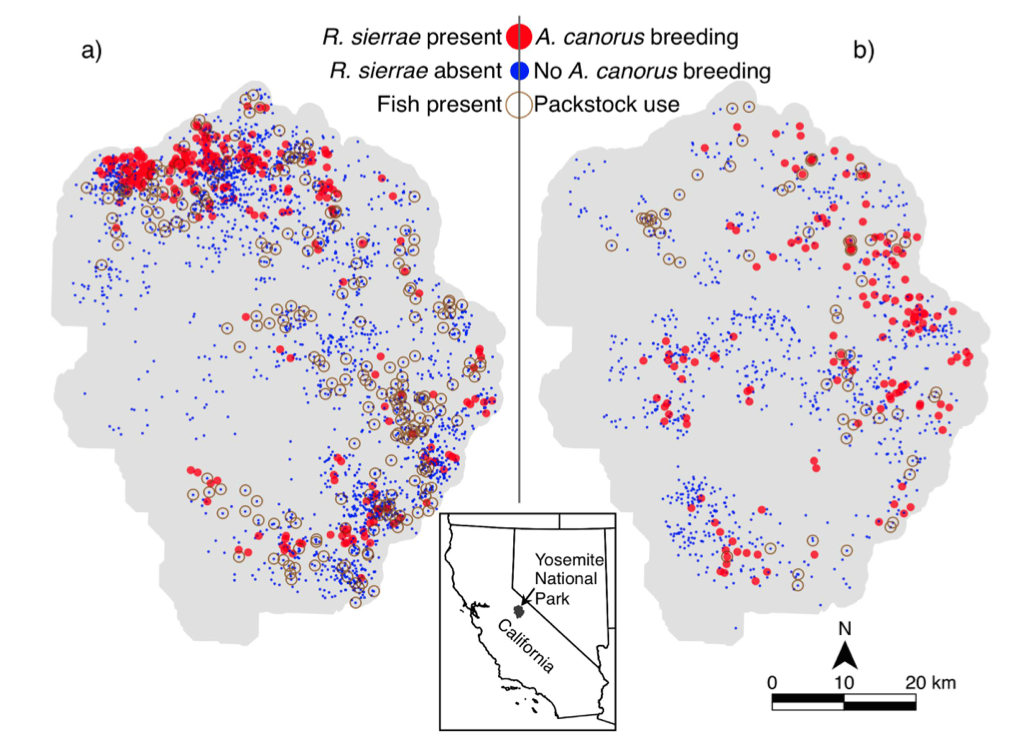
\includegraphics[width = 0.8\textwidth]{fig/toadmap.png}
\end{center}
\end{figure}


\tiny
J. R. Matchett, Philip B. Stark, Steven M. Ostoja, Roland A. Knapp, Heather C. McKenny, Matthew L. Brooks,
William T. Langford, Lucas N. Joppa, and Eric L. Berlow. Detecting the influence of rare stressors on rare species in Yosemite National Park using a novel stratified permutation test.
Scientific Reports, 5: 10702, June 2015.
}


\frame{
\frametitle{Motivating Example: Toads and Packstock}
\begin{itemize}
\itemsep15pt 
\item The response is rare (few meadows have toads).
\item The treatment is rare (few meadows are used by packstock).
\item Randomized experiment is impossible, and toad/packstock presence is not random across meadows.
\item We're interested in detecting any effect, no matter how small. If treatment effect varies across meadows, then averages might not be informative.
\end{itemize}
}

\frame{
\frametitle{Goal}
\textbf{Goal:} test the \textbf{strong null hypothesis} of no treatment effect whatsoever. \\

\begin{align*}
H_0&: Y_i(1) = Y_i(0) \text{ for all } i \\
H_1&: Y_i(1) \neq Y_i(0) \text{ for some } i
\end{align*}

\vspace{20pt}
We'd like our test to have power to detect
\begin{itemize}
\item non-constant effects
\item non-linear effects
\item effects with non-constant sign
\end{itemize}

}

\section[Matching]{Matching}

\frame
{
\frametitle{Matching}
\begin{center}
How can we estimate the counterfactual for treated individuals? \\
\vfill
\begin{itemize}
\item \textbf{Ideal:} group individuals by $X_i$ to estimate subgroup treatment effects and then average over subgroups
\item \textbf{Reality:} many covariates, perhaps continuous, make it difficult to stratify
	
\begin{center}

\begin{tikzpicture}[scale = 0.5]

\foreach \x in{0,...,4}
{   \draw (0,\x ,4) -- (4,\x ,4);
    \draw (\x ,0,4) -- (\x ,4,4);
    \draw (4,\x ,4) -- (4,\x ,0);
    \draw (\x ,4,4) -- (\x ,4,0);
    \draw (4,0,\x ) -- (4,4,\x );
    \draw (0,4,\x ) -- (4,4,\x );
}
\end{tikzpicture}
\end{center}

\item \textbf{Solution:} use a one-dimensional score to match or group individuals
\end{itemize}
\end{center}
}

\frame{
\frametitle{Propensity score matching}
$p(x)$ is usually unknown and estimated by $\hat{p}(x)$ using logistic or probit regressions
\begin{itemize}
\item Assumes a simple functional form for relationship between covariates and treatment
\item Assumes that probability of treatment takes same form for all individuals
\item May actually worsen balance if estimated incorrectly \citep{diamond_genetic_2012}
\end{itemize}
\vfill
Matching complicates inference
\begin{itemize}
\item Standard errors are difficult to compute for matching estimators \citep{abadie_large_2006, abadie_failure_2008}
\item Rarely used in hypothesis testing procedures
\item There's no ``optimal'' way to match \citep{austin_comparison_2014}
\end{itemize}

}


\subsection[Model-based Matching]{Model-based Matching}

\frame{
\frametitle{Model-based Matching}
\textbf{Idea:} Instead of modeling the propensity score, model the outcome \\
\vfill
Computing $\hat{Y}$, the ``best'' prediction of the outcome based on all covariates except for the treatment, buys us two things:

\begin{itemize} 
\item $\hat{Y}$ is a score on which to stratify observations
\item Using residuals $Y-\hat{Y}$ improves precision by removing variation due to $X$ \citep{rosenbaum_covariance_2002}
\end{itemize}
}



\frame{ 
\frametitle{Model-based Matching}
Suppose that outcomes have the form
$$Y_i(t) = f(t, X_i) + \eps_i$$
for $i = 1,\dots, N$ and $t = 0,1$. 
Let $X_i$ be fixed and suppose that $\ex(\eps_i) = 0$, independent of $X_i$ and of $\eps_j, j\neq i$. \\
\vspace{20pt}

We observe $Y_i = T_iY_i(1) + (1-T_i)Y_i(0)$. 
\vspace{20pt}

Under the strong null hypothesis, $f(0, X_i) = f(1, X_i)$ for each $i$. \\
\vspace{20pt}

Thus, our best guess of $Y_i$ needn't involve the treatment:
$$\hat{Y}_i = \hat{f}(X_i)$$

}



\frame{ 
\frametitle{Model-based Matching}
Stratify or match units on their $\hat{Y}_i = \hat{f}(X_i)$.
\vspace{10pt}
\begin{itemize}
\itemsep10pt
\item Let $S_i = j$ if unit $i$ is in stratum $j$, where $j \in \{ 1, \dots, J\}$.  Stratum $j$ contains $N_j$ units, $n_j$ of which are treated. (For now, don't worry about how to select $J$ strata.) 
\item \textbf{Under the null}, we expect units in the same strata to have the similar responses.\\
\item \textbf{Under the alternative}, the treatment adds additional information about the responses beyond $\hat{f}$.\\
The residuals will capture some of the effect of treatment:
$$ Y_i - \hat{Y}_i \not\independent T_i$$
\end{itemize}
}



\frame{
\frametitle{Permutation tests}


We will use the average difference in means across strata as our test statistic:
\vspace{30pt}
$$\tau(Y, T) =\sum_{j=1}^J  \frac{N_j}{N} \left\lvert \frac{1}{n_j} \sum_{\substack{i  : S_i = j\\T_i=1}} \left(Y_i - \hat{Y}_i \right) - \frac{1}{N_j - n_j} \sum_{\substack{i : S_i = j\\ T_i=0}} \left(Y_i - \hat{Y}_i \right) \right\rvert$$

\vspace{45pt}
\textbf{NB:} we can use any other test statistic that measures association between $Y_i - \hat{Y}_i$ and $T_i$, e.g. correlation
}

\frame{ 
\frametitle{Permutation tests}
\textbf{Basic idea:}
Under the null hypothesis, the probability distribution of the data is invariant under permutation of treatment assignments within strata. \\
\vspace{10pt}

Once we observe the actual data, we know other possible data sets that are equally likely. \\
\vspace{10pt}

There are 
$$\prod_{j=1}^J {N_j \choose n_j}$$

equally likely assignments to treatment, conditional on the strata.
}






\frame{ 
\frametitle{Permutation tests}
We approximate the null distribution using this invariance principle. \\
\vspace{10pt}
\begin{itemize}
\itemsep10pt 
\item Permute treatment assignments, independently in each stratum, to obtain new treatment vector $T_1^*$. 
\item Compute the test statistic $\tau(Y, T_1^*)$.
\item Repeat a large number $B$ times to get a distribution $\tau(Y, T_1^*), \dots, \tau(Y, T_B^*)$.
\item The p-value of the test is 

$$p = \pr(\tau(Y, T) \geq \tau(Y,  t)) \approx \frac{\sum_{i=1}^B \mathbb{I}( \tau(Y, T_b^*) \geq \tau(Y, T))}{B}$$
\end{itemize}

}



\frame{
\frametitle{Association or Causation?}

\begin{itemize}
\itemsep20pt
\item \citep{matchett_detecting_2015} concede that they're not looking for causal effects
\item Pathological example: suppose $Y_i = cT_i + \eps_i$, $X_i = T_i$. A model-based matching test will find no treatment effect.

\begin{figure}[h]
\begin{tikzpicture}
\SetGraphUnit{2} 
\Vertex{T} \SOWE(T){Y} \SOEA(T){X}
\Edges(T, Y) \Edges(T, X) 
\end{tikzpicture}
\end{figure}
\item Difference with predictive statistics: covariates included in fitting $\hat{f}$ must be pretreatment!
\end{itemize}



}


\section[Simulations]{Simulations}

\frame{
\frametitle{Simulation set-up}
$$Y_i = 1 + 2X_{1i} + 4X_{2i} + \tau_i T_i + \eps_i, \qquad i = 1, \dots, 100$$
\vspace{10pt}

\begin{itemize}
\itemsep10pt
\item $X_{1i}, X_{2i}$ are independent $\normal(0,1)$ 
\item $\eps_i$ are IID $\normal(0,1)$ (unless specified otherwise)
\item $T_i$ assigned various ways
\begin{itemize}
\item Random, independent of everything
\item Correlated with $X_1$: $T_i = \nu X_{1i} + \delta_i$, with $\delta_i \sim \normal(0,1)$
%\item Correlated with $X_1$ and $X_2$: $T_i = \nu X_{1i} + X_{1i}X_{2i} + \delta_i$, with $\delta_i \sim \normal(0,1)$
\end{itemize}
\item We vary $\tau_i$ and the method of generating $T_i$
\end{itemize}
}



\frame{
\frametitle{Results}
Model-based matching tests have correct level: random treatment assignment

\begin{figure}[htbp]
\begin{center}
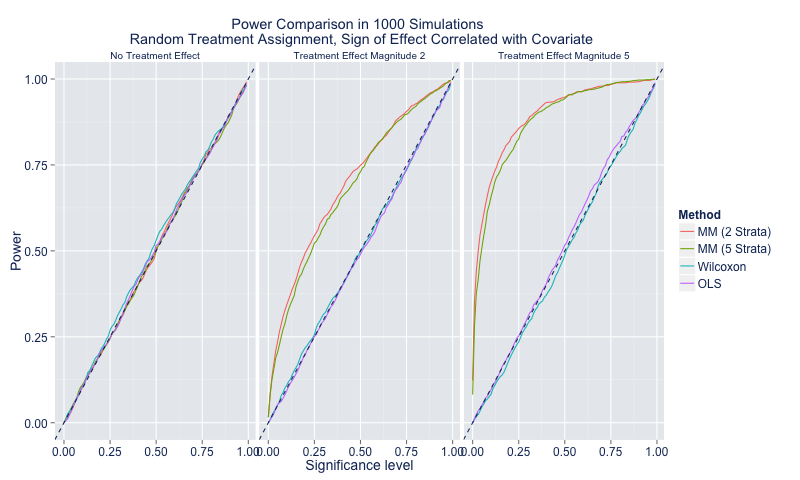
\includegraphics[width = \textwidth]{fig/power.png}
\end{center}
\end{figure}}



\frame{
\frametitle{Results}
Model-based matching tests have correct level: endogenous treatment assignment

\begin{figure}[htbp]
\begin{center}
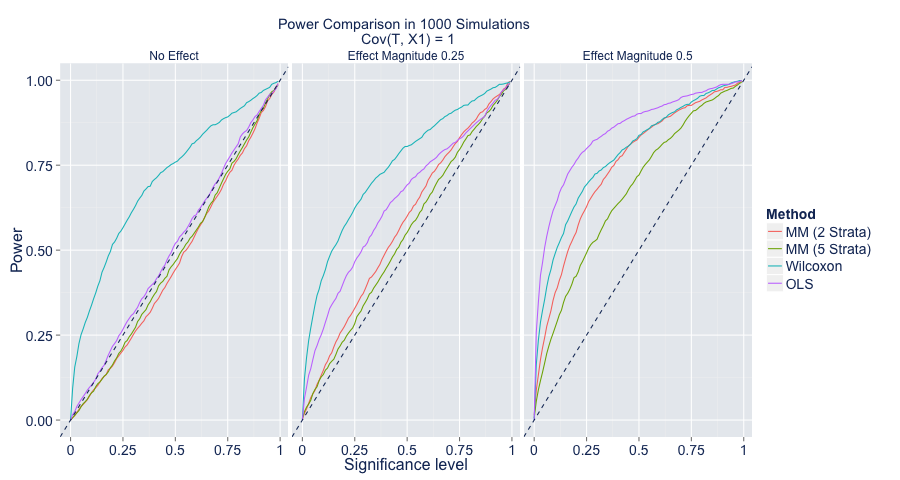
\includegraphics[width = \textwidth]{fig/power_corr.png}
\end{center}
\end{figure}}

\frame{
\frametitle{Results}
Model-based matching tests have higher power when treatment effects are non-constant

\begin{figure}[htbp]
\begin{center}
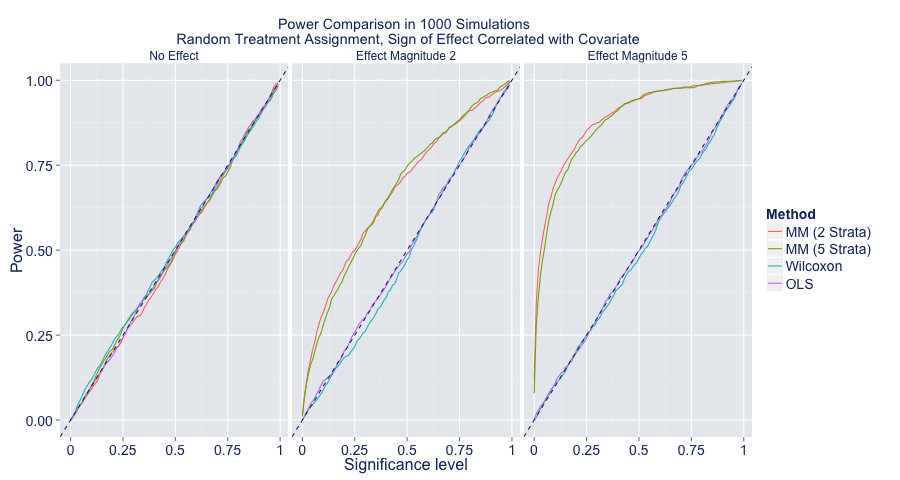
\includegraphics[width = \textwidth]{fig/power_vary_sign.png}
\end{center}
\end{figure}


}


\section[Future Directions]{Future Directions}
\frame
{
  \frametitle{Future Directions}
\begin{center}
\begin{itemize}
\itemsep20pt
\item What is the optimal way to stratify?
\item How to estimate effects and quantify uncertainty -- standard errors and confidence intervals?
\end{itemize}
\end{center}
}


\frame{
\frametitle{Stratification}
There are two competing forces that determine optimal strata:
\vspace{20pt}
\begin{itemize}
\itemsep20pt
\item Power: we need enough variation in treatment within strata
\item Precision: we want small enough strata to capture variation in treatment effects across strata
\end{itemize}
\vspace{20pt}

\textbf{Idea:} Use machine learning to identify strata that optimize some criterion \citep{athey_recursive_2015}
}





\frame{
\frametitle{Estimation}
\textbf{Approach 1:} direct estimation
\vspace{20pt}

If selection on observables holds and we fit $\hat{f}$ using only the controls, then an unbiased estimate of ATE $\tau$ is

$$ \hat{\tau} = \frac{1}{N_t} \sum_{i: T_i = 1} (Y_i - \hat{Y}_i) - \frac{1}{N_c} \sum_{i: T_i = 0} (Y_i - \hat{Y}_i)$$


\vspace{20pt}

How can we put a standard error on this? Asymptotics...

}



\frame{
\frametitle{Estimation}
\begin{overprint}
  % on every slide (not sure if it is officially supported)
  \textbf{Approach 2:} inverting hypothesis tests\\

  \onslide<1>
\vspace{20pt}
Let $A_{\tau_0}$ be the acceptance region of a level-$\alpha$ test of the hypothesis $\tau = \tau_0$.
\vspace{20pt}


$S(X) = \{ \tau \in \reals : X \in A_\tau\}$ is a $1 - \alpha$ confidence set for $\tau$.
\vspace{20pt}

An estimate of $\tau$ is the value which minimizes the probability of rejecting the null (i.e. maximizes the p-value).

$$\tilde{\tau} = \argmax_{\tau \in \reals} \pr_\tau( X \in A_\tau ) $$



\onslide<2>
\vspace{20pt}

Under $H_0: \tau = 0$, we know both potential outcomes. For $\tau \neq 0$, we don't.\\
\vspace{20pt}

We must assume some form for the treatment effect.
\begin{itemize}
\item Typically, one assumes constant additive effect
\item We can generalize to $Y(1) = g(Y(0), \tau)$ where $g$ is invertible and monotonically increasing in $\tau$
\item How can we let effects vary across strata?
\end{itemize}  


\end{overprint}
}




\frame{
\frametitle{Estimation}
Several questions arise:

\begin{itemize}
\item What is the model of treatment effects under the alternative hypothesis?

\item Are we interested in ATE? What about
\begin{itemize}
\item $\ex(Y(1) - Y(0) \mid Y(0))$
\item $\ex(Y(1) - Y(0) \mid X)$
\item $\ex(Y(1) - Y(0) \mid S = j)$
\end{itemize}

\item Back to the original problem of how to fit $\hat{f}$
\begin{itemize}
\item Fitting to controls only gives a test with incorrect level
\item Fitting to all observations biases estimated ATE
\end{itemize}

\end{itemize}
}



\frame{
\frametitle{Fitting method}
Estimation is unbiased when we fit to controls
\begin{figure}[htbp]
\begin{center}
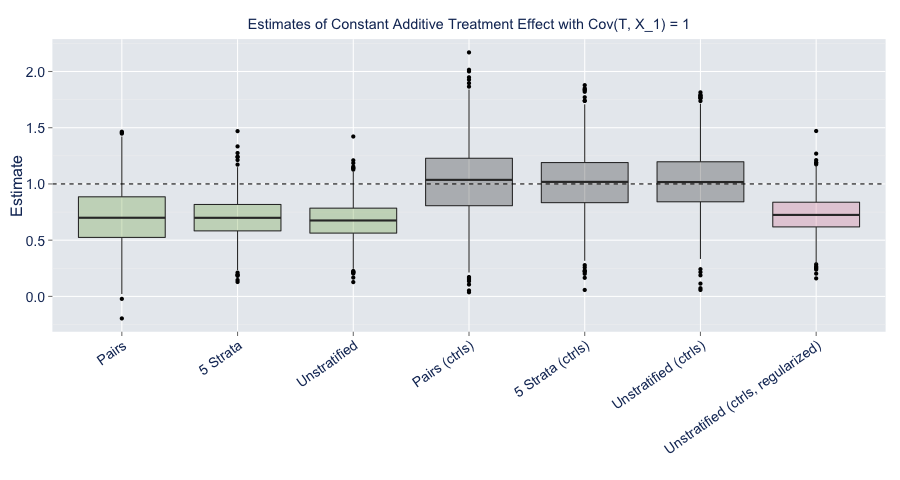
\includegraphics[width = \textwidth]{fig/est_by_fit_method.png}
\end{center}
\end{figure}
}

\frame{
\frametitle{Fitting method}
Testing has higher than nominal level when we fit to controls
\begin{figure}[htbp]
\begin{center}
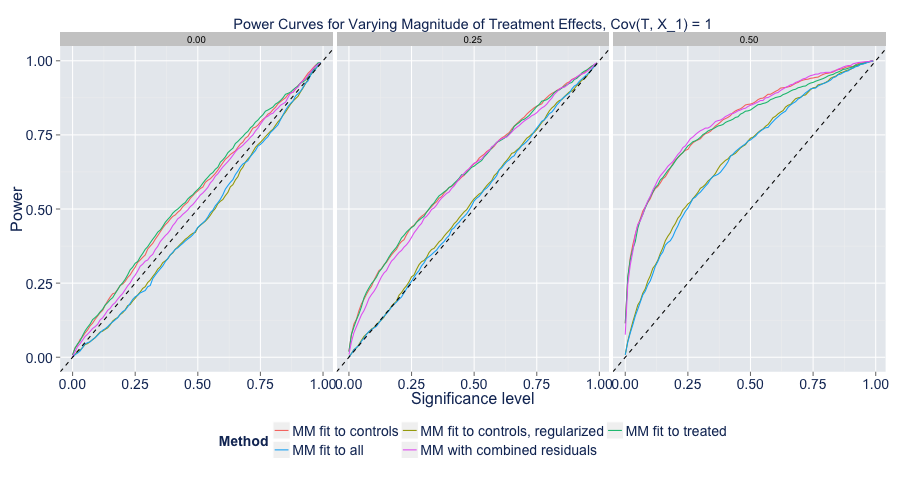
\includegraphics[width = \textwidth]{fig/power_by_fit_method.png}
\end{center}
\end{figure}

}




\frame{
\frametitle{Conclusions}
\begin{itemize}
\itemsep20pt
\item Model-based matching has higher power to detect non-constant treatment effects than traditional tests.
\item The details of modeling $\hat{Y}$ matter for getting good statistical properties and causal interpretations.
\item The methods for stratification and estimation are future work.
\end{itemize}
}

\begin{frame}
\frametitle{References}
\tiny
\bibliographystyle{plainnat}
\bibliography{refs}
\itemize
\end{frame}


\section[Appendix]{Appendix}

\frame{
\frametitle{Appendix}
\tiny

\begin{lemma}
If treatment is assigned independently across units, then $\ex\left( \frac{T_i}{N_t} \mid X\right) = \frac{1}{N}$. Likewise, $\ex\left(\frac{1-T_i}{N_c} \mid X\right) = \frac{1}{N}$, for $i = 1,\dots,N$.
\end{lemma}

\begin{proof}
\begingroup
\addtolength{\jot}{-0.5em}
\begin{align*}
\ex\left( \frac{T_i}{N_t} \mid X \right) &= \ex\left( \frac{1}{N_t} \ex(T_i \mid N_t) \right) \\
&= \ex\left( \frac{1}{N_t} \frac{N_t}{N}\right) \\
&= \frac{1}{N}
\end{align*}
\endgroup
\end{proof}
}

\frame{
\frametitle{Appendix}
\tiny

\begin{theorem}
Consider the estimator
$$ \hat{\tau} = \frac{1}{N_t} \sum_{i: T_i = 1} (Y_i - \hat{Y}_i) - \frac{1}{N_c} \sum_{i: T_i = 0} (Y_i - \hat{Y}_i)$$

If $Y(1), Y(0) \independent T \mid X$ and $0 < N_t < N$, then $\hat{\tau}$ is unbiased for the ATE.
\end{theorem}

\begin{proof}
\begingroup
\addtolength{\jot}{-0.5em}
\begin{align*}
\ex(\hat{\tau}) &= \ex\left[ \frac{1}{N_t} \sum_{i: T_i = 1} (Y_i - \hat{Y}_i) - \frac{1}{N_c} \sum_{i: T_i = 0} (Y_i - \hat{Y}_i)\right] \\
&= \ex\left[ \sum_{i=1}^N \frac{T_i(Y_i(1) - \hat{Y}_i)}{N_t} - \frac{(1-T_i)(Y_i(0) - \hat{Y}_i)}{N_c} \right] \\
&= \ex \left[ \sum_{i=1}^N \ex\left(\frac{T_i}{N_t}\mid X\right)\ex(Y_i(1) - \hat{Y}_i \mid X)- \ex\left(\frac{1-T_i }{N_c}\mid X\right)\ex(Y_i(0) - \hat{Y}_i \mid X) \right]  \\
&= \ex \left[ \sum_{i=1}^N \ex\left(\frac{T_i}{N_t}\mid X\right)\ex(Y_i(1) \mid X)- \ex\left(\frac{1-T_i }{N_c}\mid X\right)\ex(Y_i(0) \mid X) \right]  \\
&= \sum_{i=1}^N \ex\left[ \ex\left(\frac{T_i}{\sum_i T_i}\mid X\right)\right] Y_i(1) - \ex\left[ \ex\left(\frac{1-T_i }{\sum_i (1-T_i)}\mid X\right)\right] Y_i(0)    \\
&= \frac{1}{N}\sum_{i=1}^N Y_i(1)- Y_i(0)\ \\
&= ATE
\end{align*}
\endgroup
\end{proof}
}









\end{document}
